\documentclass{standalone}
\usepackage{tikz}
\usepackage{amsmath}

\begin{document}

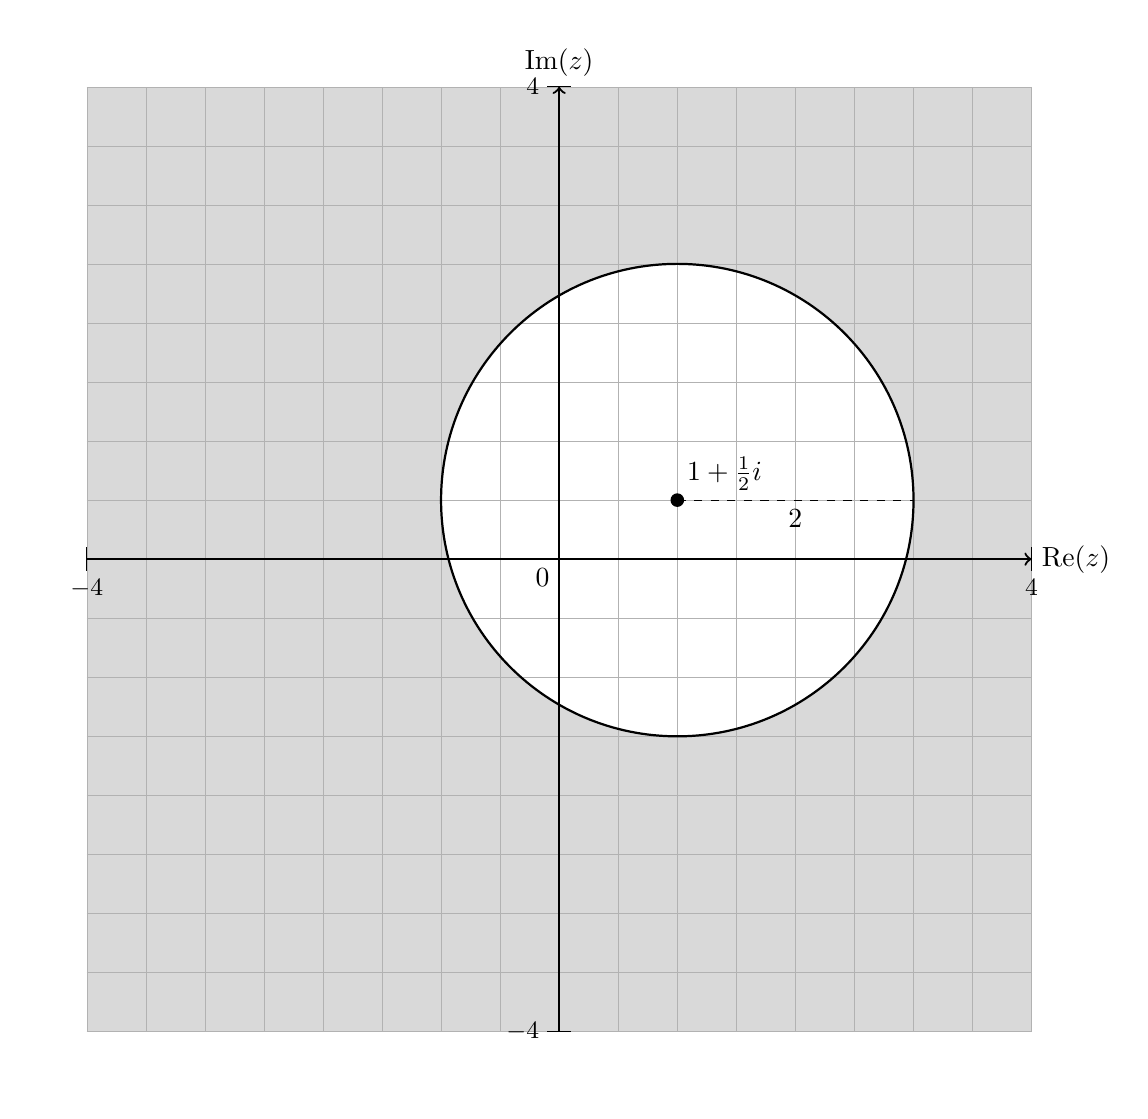
\begin{tikzpicture}[scale=1.5]
    
    % Center of the circle
    \def\xmin{-4}
    \def\xmax{4}
    \def\ymin{-4}
    \def\ymax{4}
    \def\dx{.5}
    \def\dy{.5}
    \def\xminb{\xmin-\dx}
    \def\xmaxb{\xmax+\dx}
    \def\yminb{\ymin-\dy}
    \def\ymaxb{\ymax+\dy}
    \coordinate (center) at (1.0, 0.5);

    % Fill outside region
    \begin{scope}
        \clip (\xminb, \yminb) rectangle (\xmaxb, \ymaxb);
        \fill[gray!30] (\xmin, \ymin) rectangle (\xmax, \ymax);
        \fill[white] (center) circle (2);
    \end{scope}

    % Draw grid
    \draw[step=0.5, gray!60, ultra thin] (\xmin, \ymin) grid (\xmax, \ymax); % Visible grid with lighter color
    
    % Circle
    \draw[thick] (center) circle (2);
    
    % Center point
    \filldraw[black] (center) circle (1.5pt) node[above right] {$1 + \frac{1}{2}i$};
    
    % Radius line
    \draw[dashed] (center) -- ++(2, 0) node[midway, below] {$2$};
    
    % Axes
    \draw[->, thick] (\xmin, 0) -- (\xmax, 0) node[right] {$\text{Re}(z)$};
    \draw[->, thick] (0, \ymin) -- (0, \ymax) node[above] {$\text{Im}(z)$};

    % Axis ticks
    \foreach \x in {\xmin, \xmax}
        \draw (\x, -0.1) -- (\x, 0.1) node[below=8pt] {\small $\x$};
    \foreach \y in {\ymin, \ymax}
        \draw (-0.1, \y) -- (0.1, \y) node[left=8pt] {\small $\y$};

    % Labels for axes
    \node[below left] at (0, 0) {$0$};

\end{tikzpicture}

\end{document}

